\section{Introduction}

Being a huge fan of Matt and of Numperphile,
I recently watched the video \url{https://www.youtube.com/watch?v=q6L06pyt9CA},
featuring Matt Parker.  Despite Matt's infallibility, I decided to have my own
crack at the problem, in the spirit of mathematical enquiry and whatnot.

I reasoned that checking if a number is polygonal should be a roughly
\(\BigO(1)\) operation as we can find the \(n\)th term of the base-\(s\)
polygonal numbers \(P(s, n)\), which will be quadratic in \(n\), and solve it
for \(n\) with the quadratic formula, so to check if some cannonball numbers
\(C(s, n_c)\) is polygonal we just see if the corresponding \(n_p\) is an
integer. Now \(10^9\) is a fairly small number. Seeing as my CPU's clockspeed is
in the range of gigahertz, and we're just checking a tiny fraction of those
numbers as we're just computing the cannonball numbers under this limit, it
seems reasonable that this should be doable fairly fast.

I've thought about the problem of higher-dimensional stacks of cannonballs (ie
the ones formed by adding up the cannonball numbers), but I've not done anything
about it.

While I'm here I'd also like to plug square triangular numbers:
\url{https://en.wikipedia.org/wiki/Square_triangular_number}. I conjecture that
these are one of the least talked about, but coolest things in maths. For some
inexplicable reason (``````Pell's Equation''''''), if you take a convergent
\(b / c\) of \(\sqrt 2\), then \(b^2 c^2\) will be a square triangular number.
(Matt Parker voice) How cool is that?!

\section{The Maths}

Indeed, this approach does seem to work. Almost by definition we have the
recurrence in polygonal numbers
\begin{equation*}
P(s, n) = P(s, n - 1) + n(s - 2) - (s - 3)
\end{equation*}
so we can use
\begin{align*}
P(s, n) &= \sum_{r = 1}^n P(s, r) - P(s, r - 1) \\
    &= \sum_{r = 1}^n (n(s - 2) - (s - 3)) \\
    &= \frac 12 n(n + 1)(s - 2) - n(s - 3) \\
    &= \frac{n^2(s - 2) - n(s - 4)} 2
\end{align*}
Fortunately this seems to agree with what Wikipedia thinks. Now, we have
\begin{alignat*}{2}
&& 0 &= (s - 2)n^2 - (s - 4)n - 2P(s, n) \\
&\implies& n &= \frac{s - 4 + \sqrt{(s - 4)^2 + 8(s - 2)P(s, n)}}{2s - 4}
\end{alignat*}
Wikipedia still seems to think we're on track.

Another result that I don't really use is that
\begin{align*}
C(s, n) &= \sum_{r = 1}^n P(s, n) \\
    &= \frac 12 \sum_{r = 1}^n (n^2(s - 2) - n(s - 4)) \\
    &= \frac 12 \pqty{\frac{n(n + 1)(2n + 1)(s - 2)} 6
                    - \frac{n(n + 1)(s - 4)} 2} \\
    &= \frac 1{12}n(n + 1)\bqty{(2n + 1)(s - 2) - 3(s - 4)}
\end{align*}
In fact I've only used this in verification of the results.

Regardless, now we need only work our way up the \(C(s, n)\)s using the
recurrence \(C(s, n) = P(s, n) + C(s, n - 1)\), and check for each if the
quadratic formula gives an integer result. This is most easily done by checking
if the discriminant is a perfect square and then checking that the denominator
divides the numerator.

\section{The Programming}

For speeeeeeed I implemented this in C (although there is a long abandoned
parallel Python implementation). I used 128-bit integers to be on the safe side,
as \(10^{19}\) is a little small for my liking. This meant I had to do a lot of
messing around to get things to actually display in base 10. This program is
shown in Listing \ref{lst_c}.

Of course, an isolated source code listing is both not executable and not
necessarily helpful, but fret not as my intact source tree is in
\texttt{../src}.

I did briefly consider either implementing or importing some kind of arbitrary
precision integer arithmetic functionality, but then I decided I wasn't going to
run it on anything fast enough to have to worry about that, and I have better
things to do.

There's also a slick little progress update that gets printed to STDERR, and a
number of zsh scripts to save me typing.

I also have a program that verifies results, removes duplicates and formats them
into a \LaTeX{} table (spoilers for table \ref{tab_ugly}), shown in listing
\ref{lst_py_verif}.

After having used these programs to obtain some data, and plot it and so on and
so forth as discussed in the next section, I noticed the glaring pattern with
the cannonball numbers derived from a side congruent to 2 modulo 3. By
assuming that this pattern continues, in that you can move 3 along and a little
up to get to a new cannonball polygonal number, it is easy to generate these
kinds of numbers at a preposterous rate. I wrote a little C program (listing
\ref{lst_c_2mod3} which took maybe ten minutes to hit the upper bounds of
128-bit integer arithmetic, so I for now I've written a Python program to bear
the torch, and painstakingly squeeze out every last member of the congruence
class at my leisure.

\begin{longlisting}
\inputminted{c}{../src/c/cannonball.c}
\caption{The main C source code}
\label{lst_c}
\end{longlisting}

\begin{longlisting}
\inputminted{python}{../src/factcheck.py}
\caption{Python verification program}
\label{lst_py_verif}
\end{longlisting}

\begin{longlisting}
\inputminted{c}{../src/c/2mod3/2mod3.c}
\caption{C program to find cannonball polygons for side congruent to 2 mod 3}
\label{lst_c_2mod3}
\end{longlisting}

\section{The Ugly}

I have plotted both the data in its entirety on a double logarithmic scale
\ref{fig_log_all}.

The obvious pattern that jumps out is the big line of points for all the sides
congruent to \(2 \pmod 3\). Particularly because it looks like such a straight
line on the log-log plot, we would expect it to be modelled well as a constant
multiple of some power of \(s\). I drew two lines that seemed to roughly bound
it, and used those to extract the points on the line and then do some linear
regression on that (figure \ref{fig_log_boring}). I obtained the formula
\begin{equation*}
C = 0.006170169 \cdot s ^ { 7.000026 }
\qquad \text{Average percentage error of  0.001840273 \%}\end{equation*}

I have also plotted these points on a linear scale, demonstrating their
relationship \ref{fig_linear_boring}.

Lastly, I plotted all points other than the points along this line in figure
\ref{fig_log_interesting}.

The R code I used to achieve all this is in Listing \ref{lst_R}.

Table \ref{tab_ugly} lists some solutions that I've found, so far. The \TeX{}
source of the table is in \texttt{../src/interesting.tex}, which is derived from
\texttt{../src/c/solutions/*}.  I have deliberately omitted the ``boring''
solutions along the dense line, favouring the more flavourful, stylish and
individualistic solutions. This is pertinent as there are so many of these that
the table would literally be three order of magnitude larger if I hadn't.

There are also two tables \texttt{boring.tex} and \texttt{all.tex} containing
only the boring solutions and all solutions, respectively, but there are such a
truly mind-boggling number of boring solutions that really it's hardly any fun
looking at them.

\begin{longlisting}
\inputminted{R}{../graph/graph.R}
\caption{R graphical analysis}
\label{lst_R}
\end{longlisting}

\begin{figure}[H]
\centering
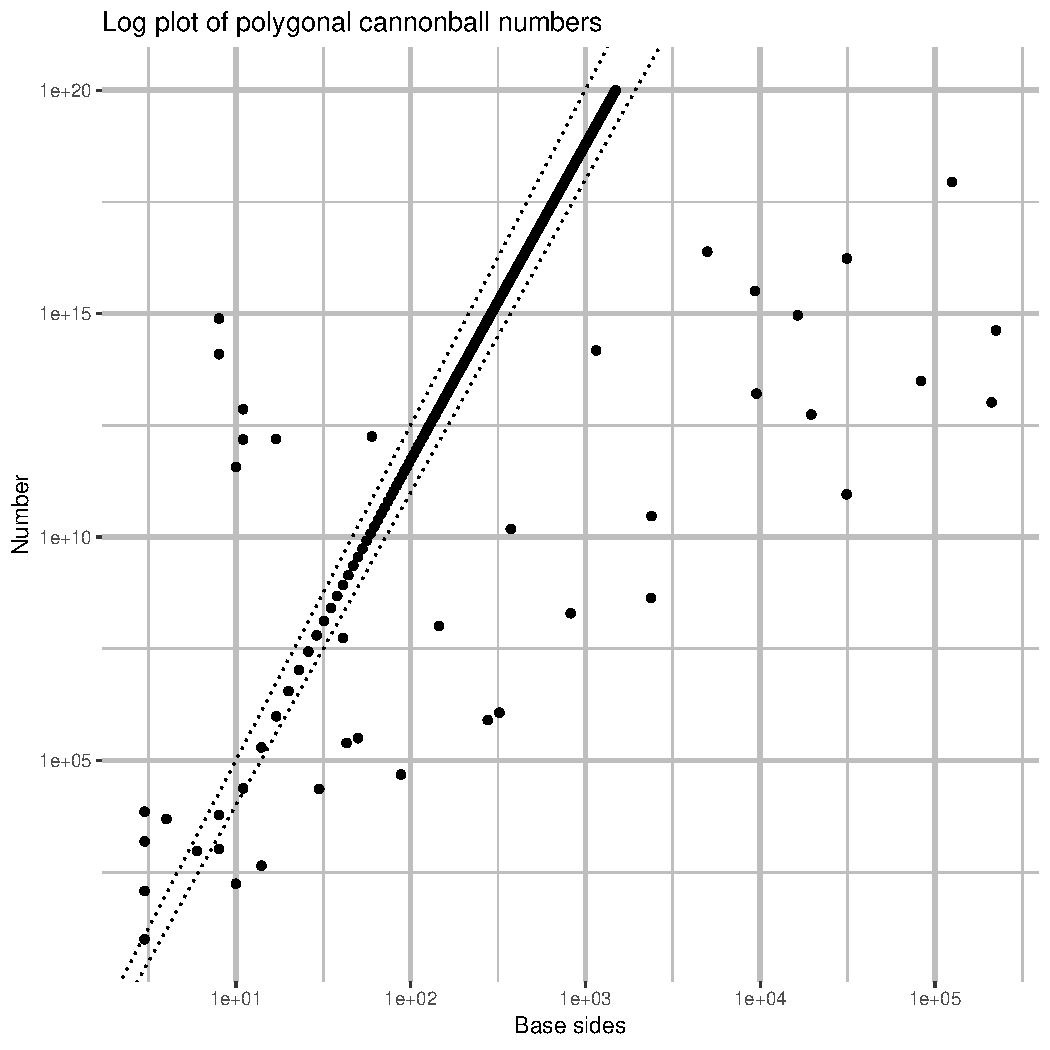
\includegraphics[width=\textwidth,page=1]{../graph/Rplots.pdf}
\caption{Log plot}
\label{fig_log_all}
\end{figure}

\begin{figure}[H]
\centering
\includegraphics[width=\textwidth,page=2]{../graph/Rplots.pdf}
\caption{Linear plot of boring points}
\label{fig_linear_boring}
\end{figure}

\begin{figure}[H]
\centering
\includegraphics[width=\textwidth,page=3]{../graph/Rplots.pdf}
\caption{Log plot of the boring points}
\label{fig_log_boring}
\end{figure}

\begin{figure}[H]
\centering
\includegraphics[width=\textwidth,page=4]{../graph/Rplots.pdf}
\caption{Log plot of the remaining points}
\label{fig_log_interesting}
\end{figure}

\begin{longtable}{*4r}
\toprule
\boldmath \(s\) & \boldmath \(C(s, n_c) = P(s, n_p)\)
& \boldmath \(n_p\) & \boldmath \(n_c\) \\
\midrule
\endhead
3 & 10 & 4 & 3 \\
3 & 120 & 15 & 8 \\
3 & 1540 & 55 & 20 \\
3 & 7140 & 119 & 34 \\
4 & 4900 & 70 & 24 \\
6 & 946 & 22 & 11 \\
8 & 1045 & 19 & 10 \\
8 & 5985 & 45 & 18 \\
8 & 123395663059845 & 6413415 & 49785 \\
8 & 774611255177760 & 16068720 & 91839 \\
10 & 175 & 7 & 5 \\
10 & 368050005576 & 303336 & 6511 \\
11 & 23725 & 73 & 25 \\
11 & 1519937678700 & 581175 & 10044 \\
11 & 7248070597636 & 1269127 & 16906 \\
14 & 441 & 9 & 6 \\
14 & 195661 & 181 & 46 \\
17 & 975061 & 361 & 73 \\
17 & 1580765544996 & 459096 & 8583 \\
20 & 3578401 & 631 & 106 \\
23 & 10680265 & 1009 & 145 \\
26 & 27453385 & 1513 & 190 \\
29 & 63016921 & 2161 & 241 \\
30 & 23001 & 41 & 17 \\
32 & 132361021 & 2971 & 298 \\
35 & 258815701 & 3961 & 361 \\
38 & 477132085 & 5149 & 430 \\
41 & 55202400 & 1683 & 204 \\
41 & 837244045 & 6553 & 505 \\
43 & 245905 & 110 & 33 \\
44 & 1408778281 & 8191 & 586 \\
47 & 2286380881 & 10081 & 673 \\
50 & 314755 & 115 & 34 \\
50 & 3595928401 & 12241 & 766 \\
53 & 5501691505 & 14689 & 865 \\
56 & 8214519205 & 17443 & 970 \\
59 & 12001111741 & 20521 & 1081 \\
60 & 1785508245600 & 248132 & 5695 \\
62 & 17194450141 & 23941 & 1198 \\
65 & 24205450501 & 27721 & 1321 \\
68 & 33535911025 & 31879 & 1450 \\
71 & 45792819865 & 36433 & 1585 \\
74 & 61704091801 & 41401 & 1726 \\
77 & 82135801801 & 46801 & 1873 \\
80 & 108110983501 & 52651 & 2026 \\
83 & 140830060645 & 58969 & 2185 \\
86 & 181692979525 & 65773 & 2350 \\
88 & 48280 & 34 & 15 \\
89 & 232323110461 & 73081 & 2521 \\
92 & 294592986361 & 80911 & 2698 \\
95 & 370651946401 & 89281 & 2881 \\
98 & 462955752865 & 98209 & 3070 \\
145 & 101337426 & 1191 & 162 \\
276 & 801801 & 77 & 26 \\
322 & 1169686 & 86 & 28 \\
374 & 15064335000 & 9000 & 624 \\
823 & 197427385 & 694 & 113 \\
1152 & 149979784926720 & 510720 & 9215 \\
2378 & 432684460 & 604 & 103 \\
2386 & 29437553530 & 4970 & 420 \\
4980 & 24264913354964425 & 3122317 & 30810 \\
9325 & 3176083959788026 & 825436 & 12691 \\
9525 & 16195753597485 & 58322 & 2169 \\
16420 & 913053565546276 & 333506 & 6936 \\
19605 & 5519583702676 & 23731 & 1191 \\
31265 & 90525801730 & 2407 & 259 \\
31368 & 17147031694579605 & 1045635 & 14858 \\
83135 & 31148407558500 & 27375 & 1310 \\
125070 & 890348736143873526 & 3773306 & 34956 \\
210903 & 10290361955160 & 9879 & 664 \\
223613 & 421687634347915 & 61414 & 2245 \\

\bottomrule
\caption{Polygonal Cannonball Numbers}
\label{tab_ugly}
\end{longtable}
